\fancychapter{Introduction}
\cleardoublepage%
% The following line allows to ref this chapter
\label{chap:intro}%



\section{Motivation}
 

\par Worldwide, there has been growing interest in the use of autonomous vehicles to execute missions of increasing complexity without constant supervision of human operators. 
\par The WiMUST project \cite{sonar_tec_overview} is an example of a project that demanded the use of such autonomous vehicles. The goal was to design a system of cooperating \acp{AMV} able to perform innovative geotechnical surveying operations. Specifically, the WiMUST system consisted of an array of physically disconnected \acp{AMV}, acting as intelligent sensing and communicating nodes of a moving acoustic network. Together, the vehicles formed a geometry formation actively controllable according to the needs of a specific application. 
\par Applications for the \ac{AMV} formation handled by the WiMUST system include seabed mapping, seafloor characterization and seismic exploration. The overall system behaves as a distributed acoustic array capable of acquiring acoustic data obtained by illuminating the seabed and the ocean sub-bottom with strong acoustic waves sent by one (or more) acoustic sources installed onboard a support ship/boat (see figure \ref{fig:WiMUST_System}). Advantages of multiple \acp{AMV} acting cooperatively as opposed to a single one include robustness against failure of a single node and improved seabed and sub-bottom resolution. They can also adapt better to unforeseen circumstances in the terrain by making better use of the larger environments that they can observe as the spatial distance between each \ac{AMV} can be varied. 
\par Another, unrelated, example of application that justifies the use of multiple autonomous vehicles was the Intel show at the 2018 Winter Olympics, where 1200 drones were used to put on a light show in the night sky. Each drone was mounted with a light bulb and, together, formed different shapes in the sky.
\par Complex systems like the two previously presented have in common the ability to properly plan motion for each vehicle that satisfies certain criteria such as simultaneous arrival of each vehicle in a formation while minimizing spent energy or time and avoiding collisions between vehicles and the environment.
\par Over the past decades, many approaches to solve motion planning problems have been proposed. Examples include bug algorithms, randomised algorithms such as PRM, RRT, RRT*, cell decomposition methods, graph-based approaches, planners based on learning, and methods based on optimal control formulations. Each technique has different advantages and disadvantages, and is best-suited for certain types of problems. Trajectory generation based on optimal control formulations stands out as particularly suitable for applications that require the trajectories to minimize (or maximize) some cost function while satisfying a complex set of vehicle and problem constraints. Finding closed-form solutions for Optimal Control problems can be difficult or even impossible to solve, and therefore numerical methods must be sought. Numerical methods can be divided into Direct and Indirect Methods. A numerical method for solving such complex Optimal Control problems consists of optimising trajectories parameterized by Bernstein polynomials \cite{lorentz2013bernstein}. Recent pioneering work on Direct Methods based on Bernstein polynomials shows interesting results \cite{cichella2018bernstein}; specifically, they can solve complex problems with a high number of vehicles while keeping computational time relatively low. The use of these methods will be further explored here.

\begin{figure}[h!]
    \centering
    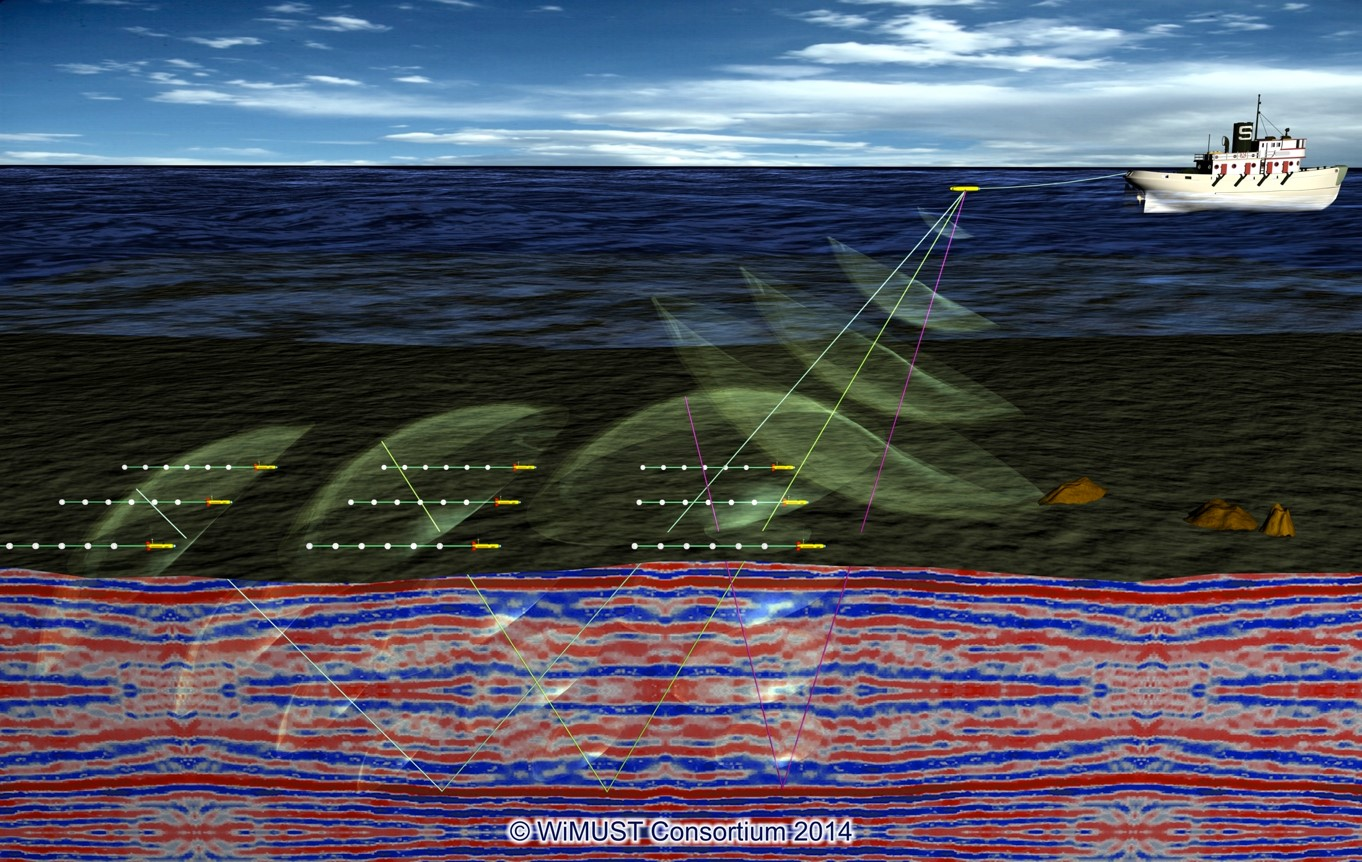
\includegraphics[width=0.5\textwidth]{Images/projects/WiMUST_project.jpg}
    \caption{Artist’s rendition of the WiMUST system for sub-bottom acoustic profiling with source-receiver decoupling}
    \label{fig:WiMUST_System}
\end{figure}


\section{Background}

\par The work discussed in this thesis focuses on motion planning for multiple cooperative vehicles. Motion Planning, as the name suggests, involves in planning of the motion of robots, such as mobile vehicles or robotic arms. Trajectory generation based on optimal control formulations are used, specifically, to solve the motion planning problems. 
\par A trajectory is a time parameterized set of states of a dynamical system. These states can be position, their derivatives, and heading, among others. The states and inputs are related to each other by a set of dynamic equations. When dealing with multiple vehicles, the trajectory optimization problem takes into account the union of states and inputs of each vehicle such that the solution describes trajectories for all of the vehicles simultaneously.
\par As discussed in the previous section, numerical solutions to the trajectory generation problems must be sought. The numerical methods can be grouped into either Direct Methods or Indirect Methods. 
\par Indirect Methods “use the necessary conditions of optimality of an infinite problem to derive a boundary value problem in ordinary differential equations” \cite{diehl2006fast}, the solutions of which must be found using analytic or numerical methods. 
\par Direct Methods, on the other hand, are based on transcribing infinite optimal control problems into finite-dimensional \acp{NLP} using some kind of paramerisation (e.g., polynomial approximation or piecewise constant parameterization). They can be solved using ready-to-use NLP solvers (e.g. MATLAB) and do not require the computation of co-state and adjoint variables as Indirect Methods do.
\par The focus on the work of this project is on the use of Direct Methods. Several parameterization methods are explored, such as piece-wise constants inputs, polynomials, and the use of Bernstein polynomials.
\par When solving an optimization problem, a model must be chosen for each vehicle. 
Different models are defined by different numbers of states and inputs and different dynamic equations. The choice of model will affect the complexity of the optimization problem. However, if the model is too simple, it may not accurately describe the real vehicle's dynamics. The Direct Methods that are tested focus on two models, the Medusa model \cite{abreu2016medusa} or the simpler Dubins' Car model \cite{Reeds1990OPTIMALPF}.


\section{Objectives}

\par The work presented in this thesis focuses on the use of Direct Methods.
\par There are several Direct Methods for trajectory optimization, for example, single and multiple shooting, collocation and quadratic programming. However, polynomial methods based on Bézier curves are particularly advantageous because they have favourable geometric properties which allow the efficient computation of the minimum distance between trajectories. As the complexity of the polynomials increases, the solutions converge to the optimal. \cite{cichella2018bernstein}
\par An Optimal Control Problem's cost can be constructed based on several criteria such as consumed energy. For \textit{cooperative} motion planning, the cost will have to be constructed differently because it will have to take into account the motion of the multiple vehicles at once, in particular, possible inter-vehicle collision.
\par The objectives of this work include
\begin{itemize}
    \item testing of methods for obstacle avoidance;
    \item comparison of different parameterization methodologies;
    \item analysis of the complexity of increasing order and number of vehicles;
    \item viability testing for non differentially flat systems;
    \item testing of the use of log barrier functions for improved computation time.
\end{itemize}


\section{Thesis Outline}

This thesis is organized as follows.  In Chapter \ref{chap:theory}, a number of direct optimization methods are presented, together with a simple motivating example that compares these methods. Chapter \ref{chap:autonomousvehiclemodels} introduces the two autonomous marine vehicle models that were used along with the simplifications adopted appropriate for the motion planning algorithms that were developed. Chapter \ref{chap:implementation} presents a formulation of the motion planning problem in the form of an equivalent optimization problem and the mathematical tools to solve it. Some results for particular motion planning problems are presented in chapter \ref{chap:results}. Finally, chapter \ref{chap:conclusion} summarizes the main achievements of the thesis and discusses topics that warrant future work.

